\documentclass[12pt,a4paper]{article}

\usepackage{xeCJK}
\usepackage{amsmath,amsthm,amssymb}
\usepackage{hyperref}
\usepackage{graphicx}
\usepackage{xcolor}
\usepackage{float}
\usepackage{makeidx}
\usepackage{listings} 
\usepackage[numbers,sort&compress]{natbib}
\usepackage[level]{datetime}
\usepackage[top=1.5cm, bottom=2cm, outer=1.5cm, inner=2cm, heightrounded, marginparwidth=0cm, marginparsep=0cm]{geometry}
%\usepackage{showframe}

\renewcommand{\today}{\number\year 年 \number\month 月 \number\day 日}
\renewcommand{\refname}{参考文献}
\renewcommand{\tablename}{表}

\newcommand{\upcite}[1]{\textsuperscript{\textsuperscript{\cite{#1}}}}
\newcommand{\tabincell}[2]{\begin{tabular}{@{}#1@{}}#2\end{tabular}}

\definecolor{dkgreen}{rgb}{0,0.6,0}
\definecolor{gray}{rgb}{0.5,0.5,0.5}
\definecolor{mauve}{rgb}{0.58,0,0.82}
\lstset{ %
  language=c++,                   % the language of the code
  basicstyle=\footnotesize,       % the size of the fonts that are used for the code
  % numbers=left,                   % where to put the line-numbers
  numberstyle=\tiny\color{gray},  % the style that is used for the line-numbers
  stepnumber=2,                   % the step between two line-numbers. If it's 1, each line 
                                  % will be numbered
  numbersep=5pt,                  % how far the line-numbers are from the code
  backgroundcolor=\color{white},  % choose the background color
  showspaces=false,               % show spaces adding particular underscores
  showstringspaces=false,         % underline spaces within strings
  showtabs=false,                 % show tabs within strings adding particular underscores
  frame=single,                   % adds a frame around the code
  rulecolor=\color{black},        % if not set, the frame-color may be changed on line-breaks within not-black text (e.g. commens (green here))
  tabsize=2,                      % sets default tabsize to 2 spaces
  captionpos=b,                   % sets the caption-position to bottom
  breaklines=true,                % sets automatic line breaking
  breakatwhitespace=false,        % sets if automatic breaks should only happen at whitespace
  % title=\lstname,                 % show the filename of files included with \lstinputlisting;
                                  % also try caption instead of title
  keywordstyle=\color{blue},      % keyword style
  commentstyle=\color{dkgreen},   % comment style
  stringstyle=\color{mauve},      % string literal style
  escapeinside={\%*}{*)},         % if you want to add LaTeX within your code
  morekeywords={*,...}            % if you want to add more keywords to the set
}

\title{第二节课习题}
\author{高洪臣}
\date{2019年6月23日}

\begin{document}

\maketitle

\section*{基础作业}

\begin{enumerate}

\item 设置IMU仿真代码中的不同参数,生成Allan方差\cite{variance2015noise}曲线

(1)参数1

在IMU仿真代码 vio\_data\_simulation(ros version) 中设置参数,生成bag文件

\begin{lstlisting}[frame=shadowbox]
double gyro_bias_sigma  = 0.00005;
double acc_bias_sigma   = 0.0005;
double gyro_noise_sigma = 0.015; // rad/s
double acc_noise_sigma  = 0.019; // m/(s^2)
\end{lstlisting}

根据生成的bag文件,通过 imu\_utils 生成Allan方差曲线

\begin{figure}[htbp] 
\centering
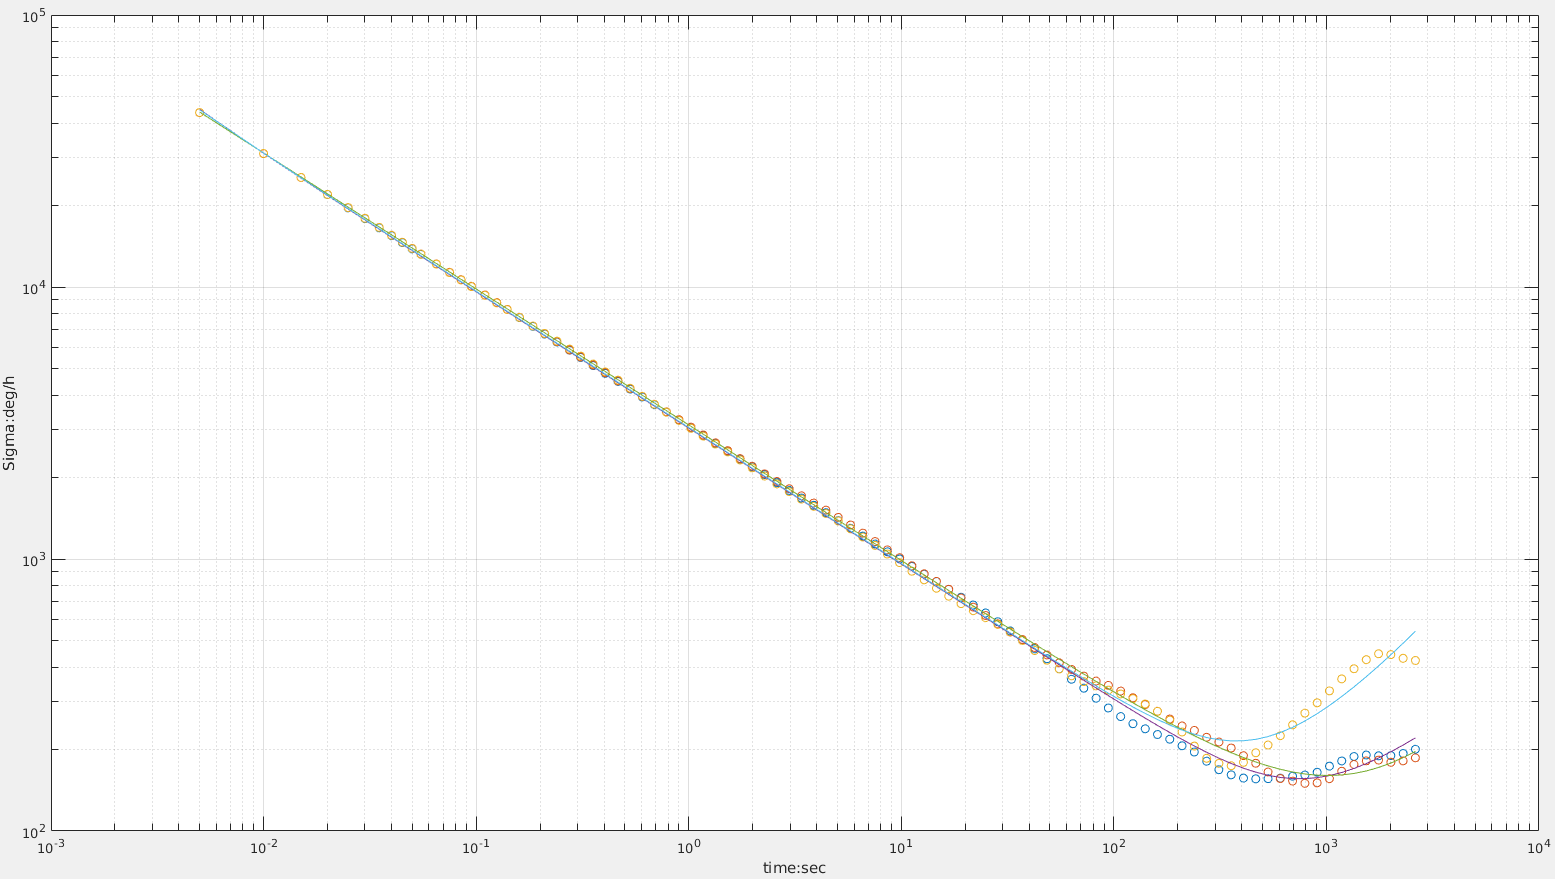
\includegraphics[width=15cm]{imu_sim_01_gyr.png} 
\caption{AD log-log plot of Gyroscope}
\label{fig:ad11} 
\end{figure} 

根据Allan方差曲线\ref{fig:ad11},$
\sigma_g = 3007     \; \frac{deg}{h} \frac{1}{\sqrt{hz}} 
         = 0.014578 \; \frac{rad}{s} \frac{1}{\sqrt{hz}}
$,$\sigma_{bg}$ 的数量级在 $10^{-5}$;

\begin{figure}[htbp] 
\centering
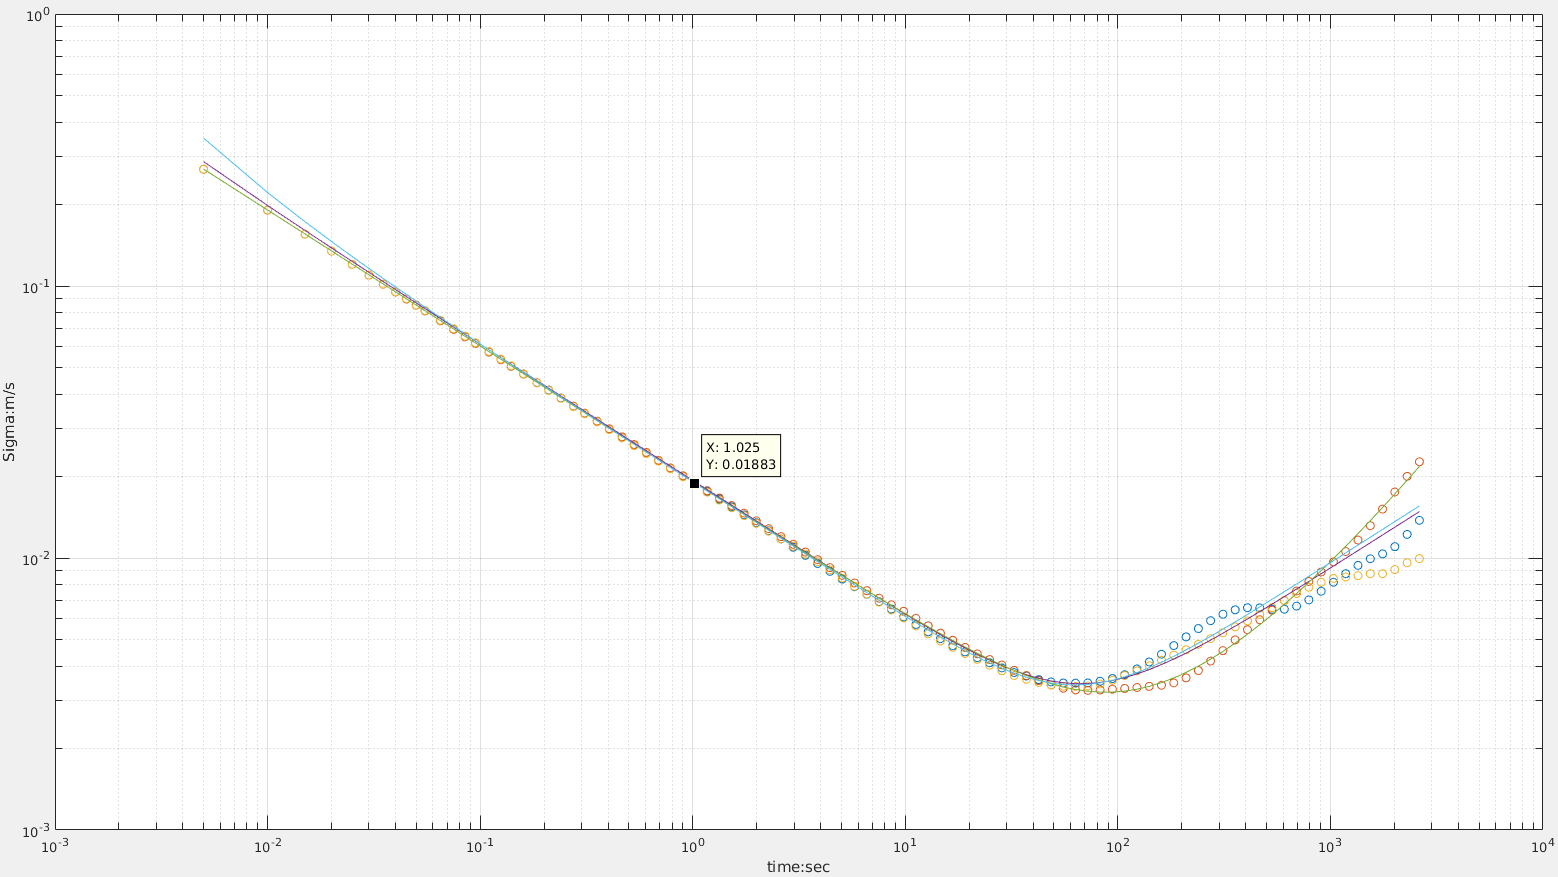
\includegraphics[width=15cm]{imu_sim_01_acc.png} 
\caption{AD log-log plot of Acceleration}
\label{fig:ad12} 
\end{figure} 

根据Allan方差曲线\ref{fig:ad12},$\sigma_a = 0.01883\;\frac{m}{s^2}\frac{1}{\sqrt{hz}}$,$\sigma_{ba}$ 的数量级在 $10^{-4}$。


\newpage

(2)参数2

在IMU仿真代码 vio\_data\_simulation(ros version) 中设置参数,生成bag文件

\begin{lstlisting}[frame=shadowbox]
double gyro_bias_sigma  = 0.00001;
double acc_bias_sigma   = 0.0001;
double gyro_noise_sigma = 0.005;  // rad/s
double acc_noise_sigma  = 0.0003; // m/(s^2)
\end{lstlisting}

根据生成的bag文件,通过 imu\_utils 生成Allan方差曲线

\begin{figure}[htbp] 
\centering
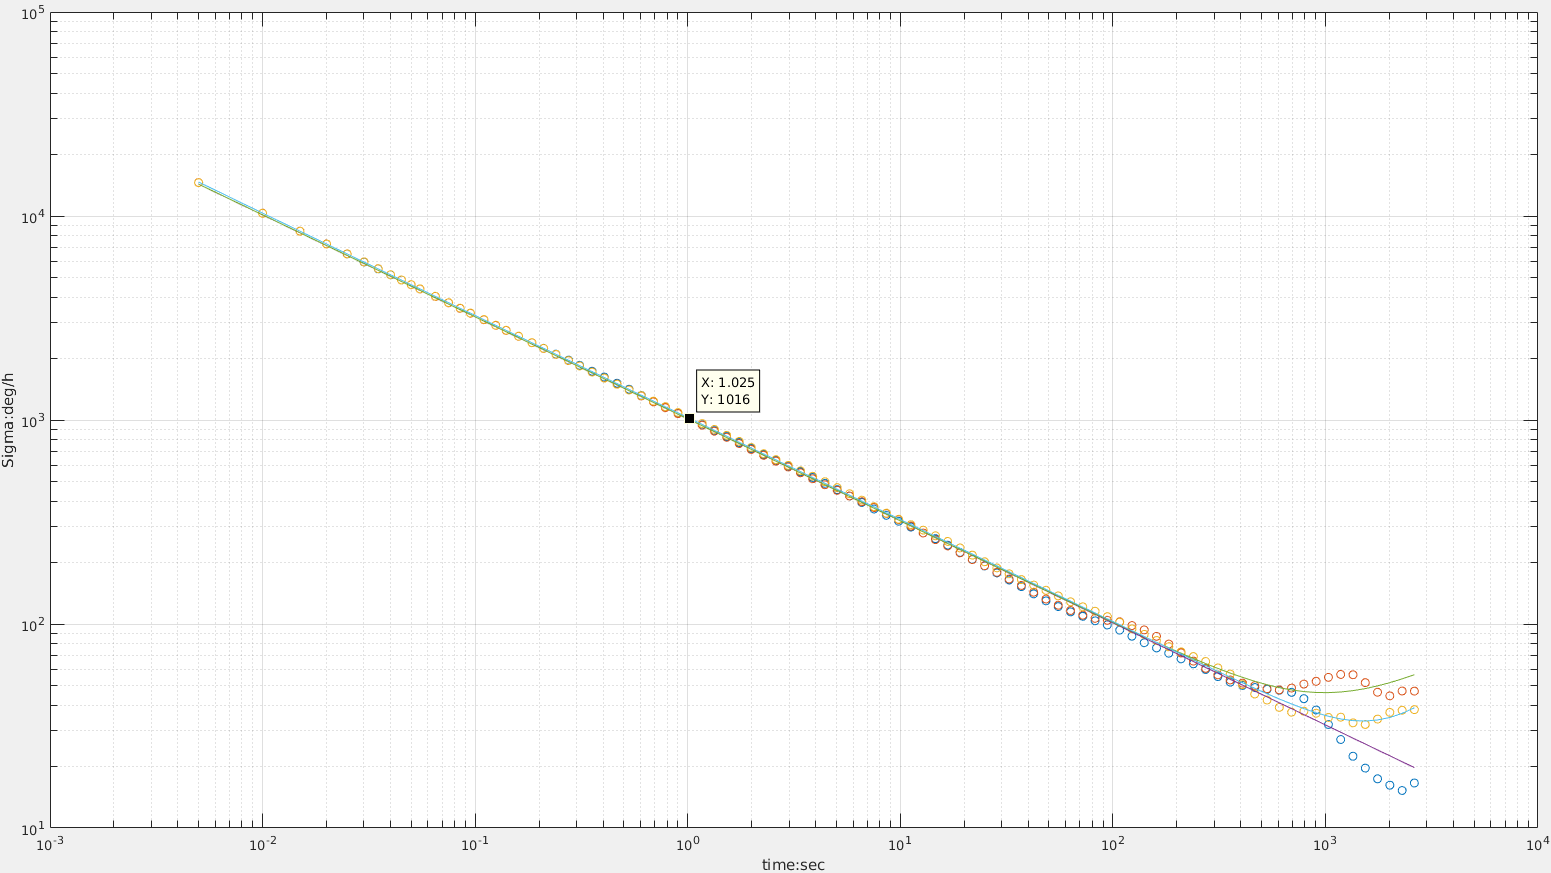
\includegraphics[width=15cm]{imu_sim_02_gyr.png} 
\caption{AD log-log plot of Gyroscope}
\label{fig:ad21} 
\end{figure} 

根据Allan方差曲线\ref{fig:ad21},$
\sigma_g = 1016    \; \frac{deg}{h} \frac{1}{\sqrt{hz}} 
         = 0.0049  \; \frac{rad}{s} \frac{1}{\sqrt{hz}}
$,$\sigma_{bg}$ 的数量级在 $10^{-5}$;

\begin{figure}[htbp] 
\centering
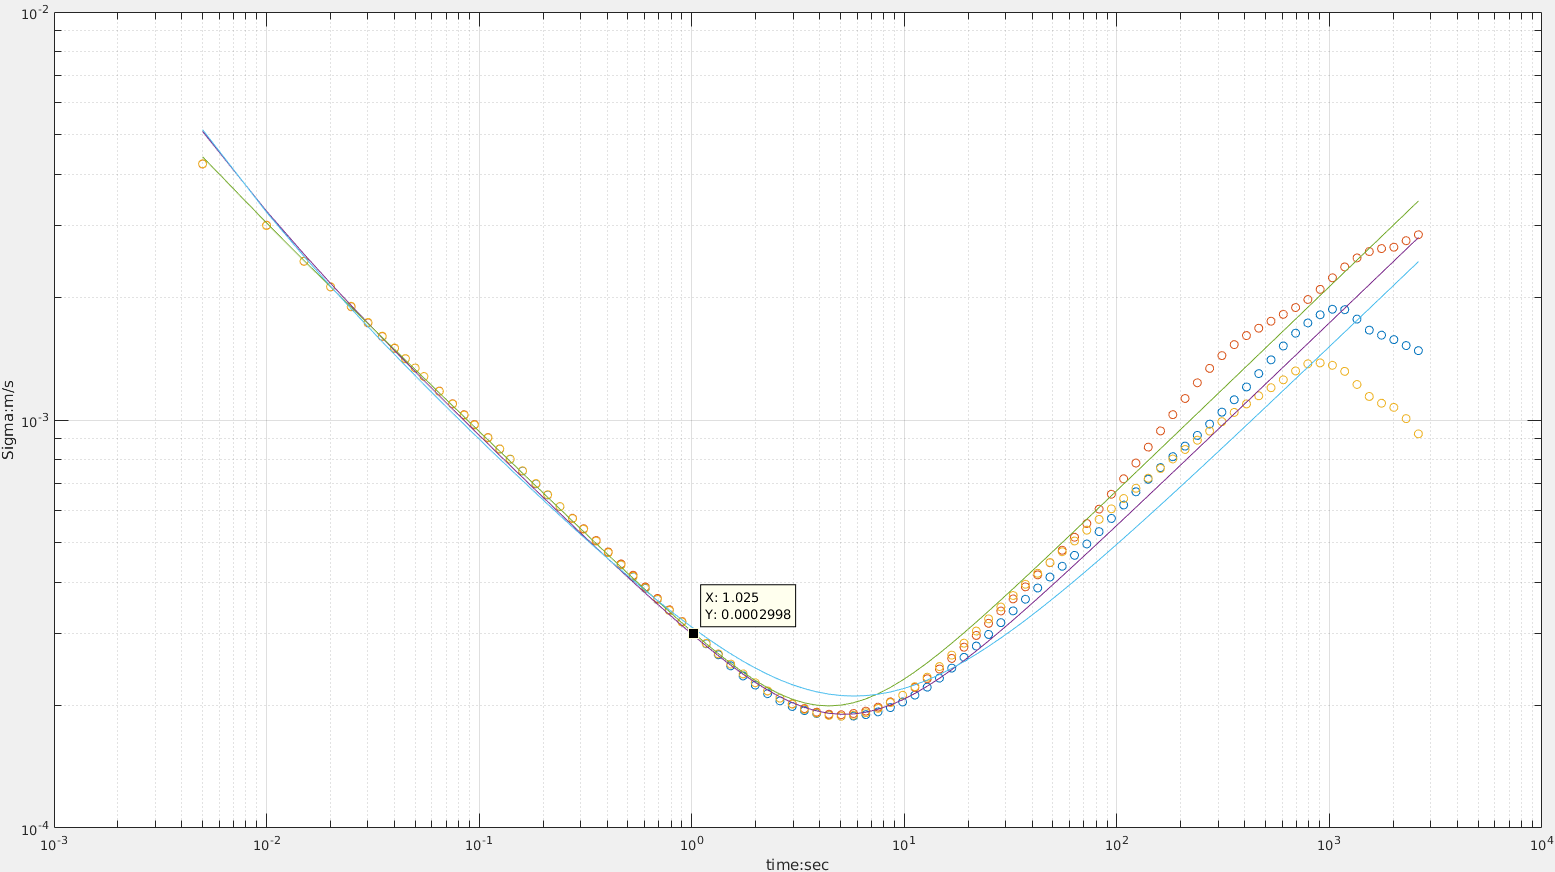
\includegraphics[width=15cm]{imu_sim_02_acc.png} 
\caption{AD log-log plot of Acceleration}
\label{fig:ad22} 
\end{figure} 

根据Allan方差曲线\ref{fig:ad22},$\sigma_a = 0.0002998 \;\frac{m}{s^2}\frac{1}{\sqrt{hz}}$,$\sigma_{ba}$ 的数量级在 $10^{-4}$。




\newpage

\item 将IMU仿真代码中的欧拉积分替换成中值积分

\begin{lstlisting}[title=中值积分代码, frame=shadowbox]
MotionData imupose   = imudata[i];
MotionData imupose_p = imudata[i-1];

Eigen::Vector3d imu_gyro_c = imupose.imu_gyro;
Eigen::Vector3d imu_gyro_p = imupose_p.imu_gyro;

Eigen::Vector3d imu_acc_c = imupose.imu_acc;
Eigen::Vector3d imu_acc_p = imupose_p.imu_acc;

Eigen::Quaterniond dq;
Eigen::Vector3d dtheta_2 = (imu_gyro_c + imu_gyro_p) * dt * 0.25;
dq.w() = 1;
dq.x() = dtheta_2.x();
dq.y() = dtheta_2.y();
dq.z() = dtheta_2.z();

Eigen::Quaterniond Qwb_p = Qwb;
Qwb = Qwb_p * dq;

Eigen::Vector3d acc_w_c = Qwb   * imu_acc_c + gw;
Eigen::Vector3d acc_w_p = Qwb_p * imu_acc_p + gw;
Eigen::Vector3d acc_w = 0.5 * (acc_w_c + acc_w_p);

Pwb = Pwb + Vw * dt + 0.5 * dt * dt * acc_w;

Vw = Vw + acc_w * dt;
\end{lstlisting}

\end{enumerate}


\newpage

\section*{提升作业}

\noindent

阅读从已有轨迹生成 imu 数据的论文,撰写总结推导:\\

已知 $k$阶($k-1$次)B样条(B-spline)曲线的表达式\cite{qinghua1998Graphics},\cite{lovegrove2013spline}为:

\begin{equation}\label{equ:bspline}
P(t) = \sum_{i=0}^n P_i B_{i,k}(t), 
\quad s.t. \quad 
P_i \in \mathbb{R}^N, t \in [t_{k-1}, t_{n+1})
\end{equation}

其中,$P_i \in \mathbb{R}^N$ 为在时刻 $t_i$ ($i \in {0,1,\dots,n}$)的控制点,$B_{i,k}$ 为B样条基函数,其DeBoor-Cox递推公式为

\begin{equation}\label{equ:deboorcox}
\begin{aligned}
B_{i,1}(t) &= 
\begin{cases}
1 & \text{if} \ t\in [t_i, t_{i+1}), \\
0 & \text{otherwise}.
\end{cases} \\
B_{i,k}(t) &= \Big(\frac{t-t_i}{t_{i+k-1}-t_i}\Big) B_{i,k-1}(t) +
              \Big(\frac{t_{i+k}-t}{t_{i+k}-t_{i+1}}\Big) B_{i+1,k-1}(t), \quad k>1
\end{aligned}
\end{equation}

根据\cite{kim1995general},公式\eqref{equ:bspline}可转换成累积(Cumulative)形式,

\begin{equation}\label{equ:bspline_cumulative}
P(t) = P_0 \tilde{B}_{0,k}(t) + \sum_{i=1}^n (P_i - P_{i-1}) \tilde{B}_{i,k}(t)
\end{equation}

其中,

\begin{equation}\label{equ:basis_cumulative}
\tilde{B}_{i,k}(t) = \sum_{j=i}^n B_{j,k}(t)
\end{equation}

我们使用4阶3次($k=4$)均匀B样条曲线\cite{lovegrove2013spline},均匀时间间隔为$\Delta t$;在3次B样条中,时刻$t$的曲线受4个控制点的影响,我们定义这4个控制点为在时刻$[t_{i-1}, t_i, t_{i+1}, t_{i+2}]$。

为了方便表示,定义$s(t)$将$t_i$的控制点转换到$s_i \in [0,1,\dots,n]$

\begin{equation}
s(t)=\frac{t-t_0}{\Delta t}
\end{equation}

定义

\begin{equation}
u(t)=s(t)-s_i
\end{equation}

根据公式\eqref{equ:deboorcox}\eqref{equ:bspline_cumulative}\eqref{equ:basis_cumulative},$\tilde{\mathbf{B}}(u)$的矩阵形式

\begin{equation}\label{equ:basis_cumulative_matrix}
\tilde{\mathbf{B}}(u) = \mathbf{C} 
\begin{bmatrix}
1 \\ u \\ u^2 \\ u^3
\end{bmatrix}, \quad
\mathbf{C} = \frac{1}{6}
\begin{bmatrix}
6 & 0 &  0 &  0 \\
5 & 3 & -3 &  1 \\
1 & 3 &  3 & -2 \\
0 & 0 &  0 &  1
\end{bmatrix}
\end{equation}

定义$\tilde{\mathbf{B}}_j(u)$为$\tilde{\mathbf{B}}(u)$的第$j$个元素(起始索引为$0$),则$\tilde{\mathbf{B}}_0(u)=1$。

$\tilde{\mathbf{B}}(u)$对时间$t$的一阶和二阶导数为

\begin{equation}
\dot{\tilde{\mathbf{B}}}(u) = \frac{1}{\Delta t} \mathbf{C}
\begin{bmatrix}
0 \\ 1 \\ 2u \\ 3u^2
\end{bmatrix}
\end{equation}

\begin{equation}
\ddot{\tilde{\mathbf{B}}}(u) = \frac{1}{{\Delta t}^2} \mathbf{C}
\begin{bmatrix}
0 \\ 0 \\ 2 \\ 6u
\end{bmatrix}
\end{equation}

已知世界坐标系下的轨迹$\mathbf{T}_{wi}$,其表示形式为

\begin{equation}
\begin{aligned}
\mathbf{T}_{wi} 
&= \begin{bmatrix} \mathbf{p} & \mathbf{q} \end{bmatrix} \\
&= \begin{bmatrix} p_x & p_y & p_z & q_x & q_y & q_z & q_w \end{bmatrix}
\end{aligned}
\end{equation}

分别推导$\mathbf{p}$和$\mathbf{q}$的3次B样条曲线,根据公式\eqref{equ:bspline_cumulative}\eqref{equ:basis_cumulative_matrix} $\mathbf{p}$的B样条曲线表达式为

\begin{equation}
\mathbf{p}(u) = 
\mathbf{p}_{i-1} + \sum_{j=1}^3 (\mathbf{p}_{i+j-1} - \mathbf{p}_{i+j-2}) \tilde{\mathbf{B}}_j(u)
\end{equation}

通过指数和对数映射、替换$P$为$\mathbf{q}$、向量加法改为四元数乘法\cite{kim1995general},公式\eqref{equ:bspline_cumulative}重写为

\begin{equation}
\mathbf{q}(u) = \mathbf{q}_{i-1} 
\prod_{j=1}^3 \exp(\log(\mathbf{q}_{i+j-2}^{-1}\mathbf{q}_{i+j-1})\tilde{\mathbf{B}}_j(u))
\end{equation}

为了求加速度,先求$\mathbf{p}(u)$对时间$t$的一阶导数,

\begin{equation}
\dot{\mathbf{p}}(u) = \mathbf{p}_{i-1} + \sum_{j=1}^3 (\mathbf{p}_{i+j-1} - \mathbf{p}_{i+j-2}) \dot{\tilde{\mathbf{B}}}_j(u)
\end{equation}

则二阶导数为

\begin{equation}
\ddot{\mathbf{p}}(u) = \mathbf{p}_{i-1} + \sum_{j=1}^3 (\mathbf{p}_{i+j-1} - \mathbf{p}_{i+j-2}) \ddot{\tilde{\mathbf{B}}}_j(u)
\end{equation}

为了求角速度,再求$\mathbf{q}(u)$对时间$t$的一阶导数,

\begin{equation}
\dot{\mathbf{q}}(u) = \mathbf{q}_{i-1} 
(\dot{A}_1 A_2 A_3 + A_1 \dot{A}_2 A_3 + A_1 A_2 \dot{A}_3)
\end{equation}

其中,

\begin{equation}
A_j = 
\exp(\log(\mathbf{q}_{i+j-2}^{-1}\mathbf{q}_{i+j-1}) \tilde{\mathbf{B}}_j(u))
\end{equation}

\begin{equation}
\dot{A}_j = 
A_j \log(\mathbf{q}_{i+j-2}^{-1}\mathbf{q}_{i+j-1}) \dot{\tilde{\mathbf{B}}}_j(u)
\end{equation}

所以,IMU的加速度和角速度分别为

\begin{equation}
\mathbf{a}_m(u) =
\mathbf{R}_{wb}^T \cdot (\ddot{\mathbf{p}}(u) + g_w) + b_a
\end{equation}

\begin{equation}
\mathbf{\omega}_m(u) = 
\mathbf{R}_{wb}^T \cdot 2[\mathbf{q}^{-1}(u) \dot{\mathbf{q}}(u)]_{xyz} + b_g
\end{equation}

\bibliographystyle{unsrt}
\bibliography{bibfile}

\end{document}

